\documentclass[../proyecto.tex]{memoir}

\begin{document}

\chapter{Análisis}

Las estimaciones de los métodos Monte Carlo dependen en gran medida de la anchura del intervalo de confianza $[\mu+3\sigma, \mu-3\sigma]$. Dicha anchura se reduce con el incremento del número de muestras aleatorias pero lo hace lentamente con el consecuente incremento de tiempo de computación. Por esta razón se crean métodos alternativos conocidos como métodos de reducción de la varianza. En esta sección introducimos uno que se adecúa a nuestro problema, que utilizaremos en las todas las ejecuciones posteriores y a continuación procedemos a estudiar el efecto de la $\alpha$-asincronicidad en la evolución de algunas configuraciones.

\section{Reducción de la varianza}

El intervalo de confianza $[\mu+3\sigma, \mu-3\sigma]$ crece a medida que la iteración se aleja de la configuración inicial, de decir, la varianza aumenta. Es posible reducirla aumentando el número de simulaciones globalmente e incrementando notablemente el tiempo de cálculo. Por tanto proponemos incrementar el número de simulaciones a medida que las iteraciones aumenten. Este incremento requiere de la adición de nuevas simulaciones en cada iteración, las cuales serán escogidas aleatoriamente de las ya existentes modificando la semilla para no obtener simulaciones duplicadas. Experimentalmente hemos observado que un valor que muestra buenos resultados sin aumentar excesivamente el tiempo de cálculo es un incremento en cada iteración de una décima parte del valor inicial de simulaciones. 

Finalmente es posible observar la reducción del intervalo de confianza que conlleva dicho incremento en la \autoref{fig:33}, dónde visualizamos la evolución del promedio de células en cada iteración del juego de vida. Para el contenido de esta sección no es relevante la configuración de la que se han obtenido los datos. Cada punto representa una estimación Monte Carlo junto con el intervalo de confianza $[\mu+3\sigma, \mu-3\sigma]$.

\begin{figure}[H]
	\centering
	\begin{subfigure}[b]{0.9\textwidth} 
		\centering
    	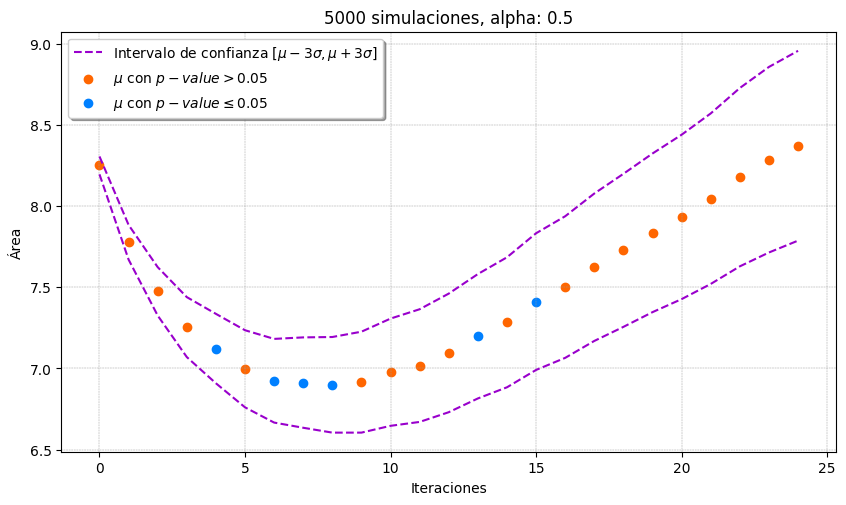
\includegraphics[width=\textwidth]{./images/iteracion_without_inc.png}
    	\caption{Ejecución sin incremento del valor inicial de simulaciones cada iteración.}
    	\label{fig:3-1}
    \end{subfigure}
    \\
	\begin{subfigure}[b]{0.9\textwidth} 
        \centering
        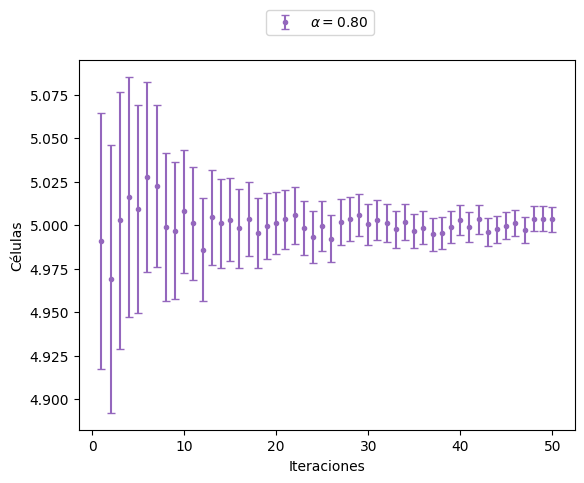
\includegraphics[width=\textwidth]{./images/iteracion_inc.png}
        \caption{Ejecución con incremento del 10\% del valor inicial de simulaciones en cada iteración.}
        \label{fig:3-2}
    \end{subfigure}
    \caption{Aplicación del método de reducción de varianza.}
    \label{fig:33}
\end{figure} 

\section{$\alpha$-asincronismo en la evolución de las configuraciones iniciales}

En esta sección vamos a estudiar el impacto de la $\alpha$-asíncronicidad. Las configuraciones iniciales son las escogidas en la sección \ref{seleccion}. Las ejecuciones son de 50 iteraciones con los valores de $\alpha$: 0.15, 0.3, 0.45, 0.6, 0.75 y 0.9. Cada iteración simulada 5000 veces aplicando el método de reducción de la varianza descrito en la sección anterior. Como resultado hemos obtenido los valores medios de las variables expuestas en la sección \ref{vars} junto con sus correspondientes intervalos de confianza para cada iteración.

\subsection{\textit{Osciladores} de periodo 2}

Comentamos los efectos de la variación de la $\alpha$-asincronicidad sobre la configuración inicial \textit{blinker}. Como se observa en la \autoref{fig:blinker_evo}, cuando no existe perturbación en el intercambio de información entre células, el calor en cada iteración es 4, es decir, 2 células mueren y 2 células nacen en cada iteración, ocupa un área de 3 \textit{nodos}$^2$ y está conformada por un solo clúster. En primer lugar, podemos observar en la \autoref{fig:4-1} que los valores de $\alpha$ se aproximan inferiormente a $0.5$, imprimen un cambio de crecimiento en el área medio. Mientras que para $\alpha=0.15$, el promedio de área a partir la vigésima iteración decrece ligeramente, para $\alpha=0.3$ el decrecimiento prácticamente desaparece, adquiriendo un valor constante y a partir de $\alpha=0.45$ comienza una acusada tendencia de crecimiento. Esta tendencia se incrementa cuando $\alpha$ se aproxima a la unidad. En particular para $\alpha=0.60$ el crecimiento a partir de la décima iteración mantiene su pendiente, hecho que no se repite para $\alpha=0.75$, donde en la vigésima iteración cambia ligeramente la pendiente y finalmente en la décimo quinta iteración de $\alpha=0.9$, el cambio de pendiente es más notable y desacelera marcadamente el crecimiento del área medio. A la vez que estos fenómenos ocurren, la iteración a partir de la cual se produce el crecimiento del área medio, decrece. Ésto es algo más visible en los valores de $\alpha$ superiores a $0.5$.

Si observamos la \autoref{fig:4-2}, contemplamos un comportamiento similar al descrito anteriormente, por tanto resulta interesante explorar el valor medio de densidad que relaciona la variación conjunta de ambas variables. 

\begin{figure}[H]
	\centering
	\begin{subfigure}[b]{0.9\textwidth} 
		\centering
    	\includegraphics[width=\textwidth]{./images/data/blinker/{Area_multiple_alpha}.png}
    	\caption{}
    	\label{fig:4-1}
    \end{subfigure}
    \\
	\begin{subfigure}[b]{0.9\textwidth} 
        \centering
        \includegraphics[width=\textwidth]{./images/data/blinker/{Celulas_multiple_alpha}.png}
        \caption{}
        \label{fig:4-2}
    \end{subfigure}
	\\
    \caption{Variación del área y número de células medio en la configuración \textit{blinker} para distintos valores de $\alpha$.}
    \label{fig:44}
\end{figure} 

El fenómeno de decrecimiento del número de iteración a partir del cual se producen los cambios descritos anteriormente, se puede visualizar más claramente en la \autoref{fig:4-3}. Cuando $\alpha$ se incrementa, la iteración a partir del cual la densidad se vuelve constante decrece. Por ejemplo, en la vigésima iteración $\alpha=0.3$ el valor medio de densidad se torna constante. Otra de las cuestiones que es posible observar sobre la variación de la densidad media es que cuando $\alpha$ crece, el valor medio de densidad constante que se alcanza se hace cada vez menor. Ésto nos informa de que durante esas iteraciones el área crece en mayor medida que el número de células, obteniéndose valores menores de densidad.

\begin{figure}[H]
	\centering
    \includegraphics[width=0.9\textwidth]{./images/data/blinker/{Densidad_multiple_alpha}.png}
    \caption{Evolución de la densidad media de la configuración \textit{blinker} para distintos valores de $\alpha$.}
    \label{fig:4-3}
\end{figure}

La \autoref{fig:5-1} muestra la variación del calor medio para distintos valores de $\alpha$. Se pueden observar dos zonas de cambio respecto a $\alpha$, una dada por los valores de $\alpha$ menores a $0.5$ y otra por los valores superiores. La primera se caracteriza por un fuerte descenso del calor hasta el rango de iteraciones 15-20, a continuación o bien se estabiliza ($\alpha=0.45$) o bien decrece ligeramente ($\alpha=0.15,0.30$). La segunda zona decrece en mucho menor medida que la anterior, hasta el rango de iteraciones 10-15 y después para $\alpha=0.6$ crece ligeramente con una pendiente constante. A diferencia de los valores $\alpha=0.75,0.90$ que la tienen más pronunciada de la décima a la vigésima iteración y a partir de esta última, cambia frenando el desacelerando del valor medio. De hecho, el calor promedio para $\alpha=0.9$ sugiere la existencia de una asíntota vertical con un calor medio igual a 3. A diferencia de los valores medios anteriormente comentados, el crecimiento que experimenta el calor cuando es mucho menos marcado y no llega a superar los valores iniciales. 

Si consultamos la \autoref{fig:5-2} que recoge la variación del número de clústeres medio respecto de $\alpha$, observamos la diferencia principal con la \autoref{fig:5-1} es que para valores de $\alpha$ mayores o iguales a $0.45$ el promedio de clústeres decrece en aproximadamente la décima iteración a un valor cercano a $0.6$, a partir de esta iteración el comportamiento es muy similar al del calor medio. En particular, el cambio de pendiente a partir de la décima iteración se reconoce unicamente para $\alpha=0.9$, mientras que para $\alpha=0.45,0.60,0.75$ la pendiente es prácticamente constante.

\begin{figure}[H]
	\centering
	\begin{subfigure}[b]{0.9\textwidth} 
		\centering
    	\includegraphics[width=\textwidth]{./images/data/blinker/{Calor_multiple_alpha}.png}
    	\caption{}
    	\label{fig:5-1}
    \end{subfigure}
    \\
	\begin{subfigure}[b]{0.9\textwidth} 
        \centering
        \includegraphics[width=\textwidth]{./images/data/blinker/{Clusteres_multiple_alpha}.png}
        \caption{}
        \label{fig:5-2}
    \end{subfigure}
	\\
    \caption{Variación del calor y número de clústeres medio en la configuración \textit{blinker} para distintos valores de $\alpha$.}
    \label{fig:55}
\end{figure}

El otro oscilador de periodo dos que hemos estudiado, la configuración \textit{toad} (\autoref{fig:toad_evo}) formada por 6 células que ocupan un área de 8 \textit{nodos}$^2$ en las iteraciones pares y 16 \textit{nodos}$^2$ en las impares, muestra un comportamiento muy similar a \textit{blinker} frente a la introducción de $\alpha$-asíncronismo en su evolución. Por ejemplo, en la \autoref{fig:66} se puede apreciar como el comportamiento es profundamente similar al mostrado en la \autoref{fig:4-2}. % no quería mal añadir aquí algo más loco, ésto está muy soso


\begin{figure}[H]
		\centering
    	\includegraphics[width=\textwidth]{./images/data/toad/{Area_multiple_alpha}.png}
    \caption{Variación del área medio en la configuración \textit{toad} para distintos valores de $\alpha$.}
    \label{fig:66}
\end{figure}

\subsection{\textit{Osciladores} de periodo 3}

\subsection{\textit{Osciladores} de periodo 4}

\subsection{\textit{Naves espaciales}}
Hasta ahora solo hemos descrito el comportamiento de \textit{osciladores}. Como se expuso en la sección \ref{spaceships}, las \textit{naves espaciales} pueden ser vistas como \textit{osciladores} que se desplazan, luego es interesante explorar si los comportamientos que hemos observado en las configuraciones iniciales anteriores se reproducen en este tipo de configuraciones iniciales. 

Comenzamos la sección estudiando la configuración inicial \textit{Lightweightspaceship} (\autoref{fig:lightweightspaceship})


Por último, la configuración inicial \textit{glider} es una nave espacial de periodo 4 formada por 5 células agrupadas en un único clúster, tiene un calor de 4 nodos y ocupa un área de 9 \textit{nodos}$^2$. Esta configuración inicial desarrolla un comportamiento sorprendentemente similar al descrito para los osciladores de periodo 2.

% Existen dos intervalos bien marcados, uno de decrecimiento (que va disminuyendo en tamaño) y otro de crecimiento que va creciendo
%\section{Efecto de la variación de la distribución de probabilidad}

%En esta sección vamos a estudiar el efecto de la generación de números aleatorios para las simulaciones utilizando distribuciones de probabilidad distintas a la uniforme. Nos resulta de especial interés algún tipo de distribución que este relacionada con el valor de $\alpha$-asincronicidad que empleemos. Una buena candidata es la distribución normal con media $\mu=\alpha$

%Cuidado, una normal centrada el $\alpha$ no da valores entre 0 y 1, hay que hacer alguna magia más


\end{document}